% IEEEAerospace2012.cls requires the following packages: times, rawfonts, oldfont, geometry
\documentclass[twocolumn,letterpaper]{IEEEAerospaceCLS}  % only supports two-column, letterpaper format

% The next line gives some packages you may find useful for your paper--these are not required though.
%\usepackage[]{graphicx,float,latexsym,amssymb,amsfonts,amsmath,amstext,times,psfig}
% NOTE: The .cls file is now compatible with amsmath!!!

\usepackage[]{graphicx}    % We use this package in this document
\usepackage{algpseudocode}
\newcommand{\ignore}[1]{}  % {} empty inside = %% comment

\begin{document}
\title{16.32 Final Report:\\ Dynamic Programming for Car Kinematics}

\author{%
Keenan Albee\\ 
Massachusetts Intsitute of Technology\\
77 Massachusetts Ave\\
Cambridge, MA 20139\\
917-531-4411\\
albee@mit.edu
}
%%%% IMPORTANT: Use the correct copyright information--IEEE, Crown, or U.S. government. %%%%%
%\thanks{\footnotesize 978-1-5386-2014-4/18/$\$31.00$ \copyright2018 IEEE}              % This creates the copyright info that is the correct 2018 data.
%\thanks{{U.S. Government work not protected by U.S. copyright}}         % Use this copyright notice only if you are employed by the U.S. Government.
%\thanks{{978-1-5386-2014-4/18/$\$31.00$ \copyright2018 Crown}}          % Use this copyright notice only if you are employed by a crown government (e.g., Canada, UK, Australia).
%\thanks{{978-1-5386-2014-4/18/$\$31.00$ \copyright2018 European Union}}    % Use this copyright notice is you are employed by the European Union.
%}


\maketitle

\thispagestyle{plain}
\pagestyle{plain}

\begin{abstract}
A dynamic programming scheme was implemented in Python to solve the optimal car motion problem. The Reeds-Shepp Car model was used over a state space $X \subset x \times y \times \theta$, with inputs $U \subset v \times \phi$. A simple collision checking algorithm was incorporated into the dynamic programming solver to allow for the placement of arbitrary rectangular obstacles in the state space. The solver was run over multiple demonstrative scenarios, including parallel parking, navigation around an obstacle, and a 180 degree turn. The algorithm runs in $O(e^n)$, where $n$ is the number of state space and input variables, in this case 5. Even taking advantage of a few heuristic tricks, this borders on the edge of feasibility due to the curse of dimensionality. Future work might involve more computationally efficient approximate solutions to the optimization problem, including RRTs.
\end{abstract}


\tableofcontents

%%%%%%%%%%%%%%%%%%%%%%%%%%%%%%%%%%%%%%
\section{Background}
\cite{LaValle1}



%%%%%%%%%%%%%%%%%%%%%%%%%%%%%%%%%%%%%%
\subsection{Dynamic Programming}

Dynamic programming provides a numerical tool for approximating optimization problems. Specifically, dynamic programming is the discrete-time approximation of the Hamilton-Jacobi-Bellman equation
\[ -J^*_t = \min_{{u \in U}} \mathcal{H} \]
and in the limit provides the exact solution for the optimal cost-to-go, $J^*$. By discretizing input actions and state, one effectively creates a mesh of state variables over which the combination of discretized state variables may be applied. \cite{Hall2018}

\subsection{Algorithm}

The dynamic programming implementation is based off of that given by 





%%%%%%%%%%%%%%%%%%%%%%%%%%%%%%%%%%%%%%%%%%%%%
\section{Method}
%%%%%%%%%%%%%%%%%%%%%%%%%%%%%%%%%%%%%%%%%%%%%
\subsection{The Reeds-Shepp Car}


\subsection{Collision Checking}

\begin{figure}[!htb]
	\begin{algorithmic}[1]
		\Procedure{Dynamic Programming}{$X,U$}
		\State $r\gets a\bmod b$
		\While{$r\not=0$}\Comment{We have the answer if r is 0}
		\State $a\gets b$
		\State $b\gets r$
		\State $r\gets a\bmod b$
		\EndWhile\label{euclidendwhile}
		\State \textbf{return} $b$\Comment{The gcd is b}
		\EndProcedure
	\end{algorithmic}
	\caption{Simple Collision Checking}\label{euclid}
\end{figure}

\subsection{Dynamic Programming}
\begin{figure}[!htb]
	\begin{algorithmic}[1]
		\Procedure{Dynamic Programming}{$X,U$}
		\State $J^*\gets h(x(t_f))$ \Comment{For admissiable final position}
		\For{$k$ iterations }\Comment{$k$ mesh iterations}
			\For{$X$ states }\Comment{discretized state}
				\For{$U$ inputs }\Comment{discretized inputs}
					\State $x_{k1}\gets f(x_k, u_k)$
		\State $b\gets r$
		\State $r\gets a\bmod b$
		\EndFor\label{euclidendwhile}
		\EndFor
		\EndFor
		\State \textbf{return} $b$\Comment{The gcd is b}
		\EndProcedure
	\end{algorithmic}
	\caption{Computational Dynamic Programming}\label{euclid}
\end{figure}

\subsection{Implementation}

\begin{figure}[!htb]
	\begin{algorithmic}[1]
		\Procedure{Euclid}{$a,b$}\Comment{The g.c.d. of a and b}
		\State $r\gets a\bmod b$
		\While{$r\not=0$}\Comment{We have the answer if r is 0}
		\State $a\gets b$
		\State $b\gets r$
		\State $r\gets a\bmod b$
		\EndWhile\label{euclidendwhile}
		\State \textbf{return} $b$\Comment{The gcd is b}
		\EndProcedure
	\end{algorithmic}
	\caption{Interpolation Logic}\label{euclid}
\end{figure}

\begin{figure*}
\centering
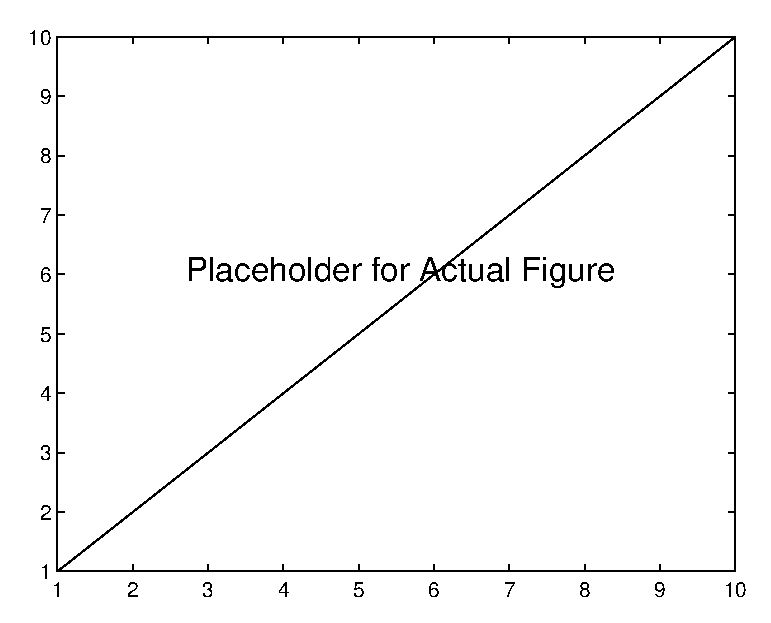
\includegraphics[width=4in]{Placeholder.eps}
\caption{\bf{Here is an example of a figure that spans both columns.}}
\label{FlowChart}
\end{figure*}


%%%%%%%%%%%%%%%%%%%%%%%%%%%%%%%%%%%%%%%%%%%%%%%%%%%%%
\section{Results}

\subsection{Computational Complexity}

\subsection{Sample Scenarios}
%%%%%%%%%%%%%%%%%%%%%%%%%%%%%%%%%%%%%%%%%%%%%%%%%%%%%
\section{Conclusions}
%%%%%%%%%%%%%%%%%%%%%%%%%%%%%%%%%%%%%%%%%%%%%%%%%%%%%

\subsection{Discussion}

\subsection{Conclusion}

%%%%%%%%%%%%%%%%%%%%%%%%%%%%%%%%%%%%%%%%%%%%%%%%%%%%%%%%%%%%%%%%%%%%%%%%%%%%%%%%%%%%%%%%%%%%%%%%%
\appendices               % note there is no {} to put a title. Each appendix has its own title
%%%%%%%%%%%%%%%%%%%%%%%%%%%%%%%%%%%%%%%%%%%%%%%%%%%%%%%%%%%%%%%%%%%%%%%%%%%%%%%%%%%%%%%%%%%%%%%%%
% For a single appendix, use the \appendix{} keyword and do not use the \section command.

\section{Dynamic Programming Algorithm}        % first appendix
%%%%%%%%%%%%%%%%%%%%%%%%%%
\begin{figure*}
	\centering
	\includegraphics[width=7.5in]{kirk_algo.png}
	\caption{\bf{The general dynamic programming algorithm. }}
\end{figure*} \cite{Kirk1971}

%%%%%%%%%%%%%%%%%%%%%%%%%%%%%%%%%%%%%%%%%%%%%%%%%%%%%%%%%%%%%%%%%%%%%%%%%%%%%%%%%%%%%%%%%%%%%%%%%%%%%%
\acknowledgments
I would like to thank Professor Hall for teaching what was a challenging, but very interesting course.
%%%%%%%%%%%%%%%%%%%%%%%%%%%%%%%%%%%%%%%%%%%%%%%%%%%%%%%%%%%%%%%%%%%%%%%%%%%%%%%%%%%%%%%%%%%%%%%%%%%%%%
\bibliographystyle{IEEEtran}
\bibliography{cite}


%%%%%%%%%%%%%%%%%%%%%%%%%%%%%%%%%%%%%%%%%%%%%%%%%%%%%%%%%%%%%%%%%%%%%%%%%%%%%%%%%%%%%%%%%%%%%%%%%%%%%%

\end{document}
